\chapter{Transcription Initiation}
Initiation is the first step in any transcription event. 
It therefore needs to be accurate in when and where it occurs. 
Transcription initiation fundamentally relies on the assembly of the \gls{pic} (a super-complex 1.5 megadaltons in size  containing \gls{pol2} \cite{fazal:2015:realtime}) on DNA.
The assembly of such complex is spatially defined by two elements: chromatin structure and core promoter elements.
Both contribute to limit the amount of spurious transcription by ensuring robust assembly of the \gls{pic} only in promoter regions.
In addition to spatial regulation, timing and intensity of transcription initiation must also be controlled.
Any specific promoter can be finely tuned by the binding of gene-specific transcription factors, that can act as either enhancers or repressors; modulating initiation efficiency either constitutively or in response to environmental effects. 
Finally, when the \gls{pic} is fully assembled, it will eventually escape the promoter and enter productive elongation.

\section{Spatial definition: Chromatin structure and core promoter elements}

Chromatin is a higher order structure that forms when DNA wraps around histones, proteins that can efficiently arrange loose DNA into compact structures.
The simplest unit of chromatin consists of 140 nucleotides of DNA tightly wrapped around a histone, forming a nucleosome.
The organization of the genome around units of nucleosomes has a moltitude of consequences, not least of which is to sterically prevent DNA binding proteins from accessing their substrate. 
As transcription relies on assembly of \gls{pol2} and the \gls{pic} on DNA to complete its initial phase, nucleosomes pose a considerable barrier to efficient initiation \cite{field:2008:distinct} \cite{jiang:2009:compiled}.
The insulation of DNA by nucleosomes has been harnessed by the cell and made into a regulatory mechanism that can spatially define where transcription initiates, as transcription factors must bind DNA for this to happen. 
To allow transcription factors to associate with DNA in promoter regions, these are always associated with an \gls{nfr}, an area of the genome where nucleosomes are depleted, leaving naked DNA available for binding.
Although certain sequence elements can passively discourage nucleosome association, several complexes can actively mediate depletion of nucleosomes from promoter regions, such as SWI1/SNF and the closely related RSC complex.
These complexes can be recruited in two ways: through sequence specificity \cite{badis:2008:library, knight:2014:two} or through recruitment by gene-specific transcription factors such as Reb1p, Abf1p, and Rap1p to promoter regions \citep{floer:2010:rscnucleosome, hartley:2009:mechanisms, spain:2014:rsc, badis:2008:library}.

While chromatin defines the position of transcription initiation, core promoter elements provide specificity for many early-acting general transcription factors. 
A number of promoter elements were identified in metazoans, where they have been shown to regulate position and intensity of transcription initiation.
Although a \gls{tss} consensus was recently defined \cite{malabat:2015:quality}, no sequence was found to be universally required for transcription initiation \cite{butler:2002:RNA}.
\cer{} promoter elements remain poorly characterized and seem to lack the majority of the sequence elements found in their metazoan counterparts. 
The major element known to bring about the assembly of the \gls{pic} in \cer{} is the TATA box.
This very short consensus sequence, TATAWAWR \citep{basehoar:2004:identification}, is present in about 15\% of yeast genes \cite{kamenova:2014:mutations} and is recognized by the \gls{tbp}, an essential factor for \gls{pic} assembly. 
At these promoters, \gls{tbp} binds DNA as part of the \gls{saga} complex, changing the conformation of DNA and priming the promoter for assembly of other general transcription factors. 
TATA-dependent promoters, however, are not the only type of promoter in \cer{}. 
The majority of yeast promoters (85-90\% )  are known as TATA-less and require binding of the TFIID complex in lieu of \gls{saga} \citep{rhee:2012:genomewide}. 
Curiously \gls{tbp}, along with a number of other shared subunits and co-factors, is also contained in the TFIID complex, but it was recently shown that, in this context, its binding activity is not required for gene activation \cite{kamenova:2014:mutations}.
TFIID and \gls{saga} have largely overlapping roles in activating gene expression, however, the predominant activity of the two complexes can be associated with functional differences.
While TFIID generally dominates over house-keeping genes that do not require regulation, \gls{saga}---and as a consequence \gls{tbp} binding---has a larger effect over highly regulated and stress-inducible genes \citep{huisinga:2004:genomewide}.
The binding of either complex represents the first step towards assembly of other general transcription factors into the \gls{pic}.

\section{Temporal definition: Gene-specific transcription factors}
While nucleosome positioning and core promoter elements define where transcription should initiate, they do not generally actively regulate it on their own.  
In the cell, many genes need to be activated in response to specific conditions or external stimuli.
These regulated genes are generally inactive and become actively transcribed only when the conditions are met.
The main mechanism that enables these transcriptional switches is the presence of gene-specific transcription factors.
These DNA-binding proteins specifically target promoter regions, modulating their activity in response to a large number of conditions.
Gene-specific transcription factors can activate---or repress---transcription in a variety of ways: activation can occur by binding DNA and recruiting NFR-generating complexes, or otherwise facilitating \gls{pic} assembly, and even by relocating chromatin to the nuclear periphery \citep{randisehinchliff:2016:transcription}.
Alternatively, transcription factors can constitutively repress their target genes and selectively lose the DNA-binding capability under certain conditions, such as the presence of a ligand.

Genome-wide studies on transcription factor organization highlighted the combinatorial potential that emerges when several transcription factors interact with the same promoters \cite{harbison:2004:transcriptional}.
Regulation of a single promoter by several distinct transcription factors can exploits their different requirements---qualitative or quantitative--- to force the emergence of complex regulatory logic.

\section{PIC assembly and promoter clearance}

Assembly of the \acrlong{pic} starts with the binding of either TFIID or \gls{saga} to promoter DNA.
The presence of \gls{tbp} in these complexes modifies the structure of DNA, allowing the step-wise recruitment of several general transcription factors and of \gls{pol2} \citep[For review see][]{sainsbury:2015:structural}.

TFIIA and TFIIB are the first factors to make contact with TBP, stabilising its interaction with DNA.
However, while TFIIA simply acts as an auxiliary factor and is dispensable \citep{imbalzano:1994:transcription}, TFIIB is required for \gls{pol2} recruitment \citep{bushnell:2004:structural}.
The presence of TFIIB  acts as a platform for TFIIF docking. 
The addition of TFIIF has the double effect of recruiting \gls{pol2} to active promoters (\gls{pol2} is bound to TFIIF when in free form \citep{rani:2004:rna}) and of further stabilising the whole \gls{pic}. 
Despite the inclusion of \gls{pol2} in the forming \gls{pic}, at this stage promoter DNA is firmly wound-up in a double helix and therefore 
%positioning of this figure is messy, play around. know that if you insert a figure with no space
%between the text the compiler will not separate the paragraph.
\begin{wrapfigure}{}{0.4\textwidth}
\centering
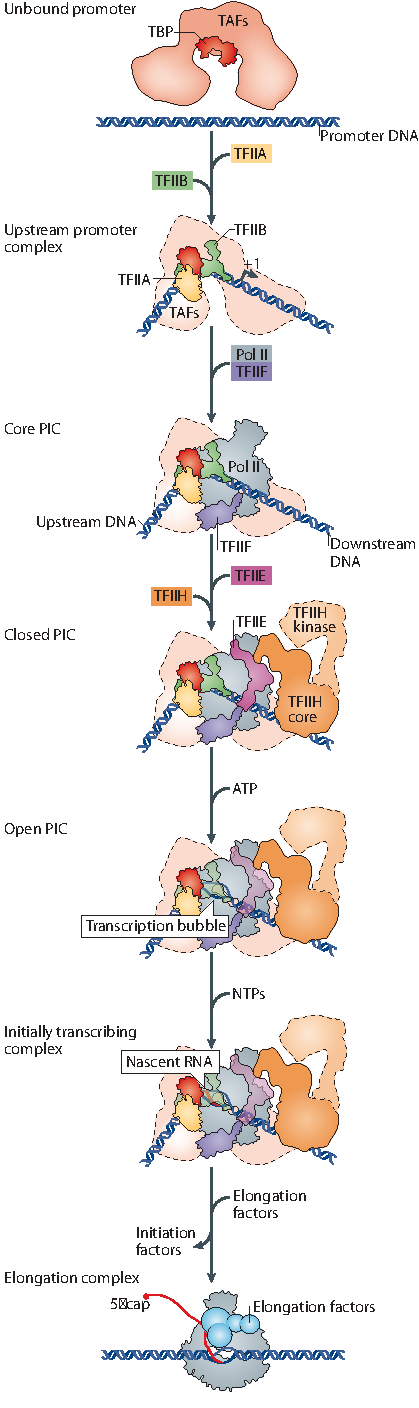
\includegraphics[width=5.095cm]{figures/introduction/picAssembly} % 5.094cm
\caption[Stepwise PIC assembly]{
Stepwise assembly of general transcription factors and \gls{pol2} on a promoter.
adapted from \cite{sainsbury:2015:structural}.
}
\label{fig:picAssembly}
\centering
\end{wrapfigure}
the ternary complex\footnote{The ternary complex is defined as the three-way interaction between DNA, RNA, and \gls{pol2} that forms within transcribing polymerases} required for transcription cannot yet form.
TFIIE and TFIIH are recruited to the \gls{pic} to solve this problem.
TFIIE acts as a bridge between \gls{pol2} and TFIIH, who contains an ATPase module and is able to unwind promoter DNA \citep{holstege:1996:opening}.
This will eventually contribute to DNA melting and the formation of the open \gls{pic}, a structural variant that precedes the shift into elongation.



The order of stepwise assembly of general transcription factors into a functional \gls{pic} was first discovered \invitro{} \cite{buratowski:1989:five}. 
\Invivo{}, however, there is evidence for the activity of the mediator complex in providing additional assembly pathways \cite{esnault:2008:mediatordependent}.
Mediator is a large and flexible protein complex that can interact with virtually every general transcription factor and with \gls{pol2}.
It is known for its fundamental role in transducing regulatory signals from gene-specific transcription factors to the polymerase.
Without Mediator, the \gls{pic} can drive basal transcription levels, but its activity cannot be modulated in response to external factors.
Studies have implicated mediator in the recruitment of TFIIE and TFIIH independently of \gls{pol2}, providing alternative ways to assemble the complete \gls{pic}.
Additionally, interactions between \gls{pol2} and mediator were found to be required for transcription \invivo{} \cite{soutourina:2011:direct}.

After the assembly of the \gls{pic} and the Mediator complex on the promoter, \gls{pol2} relies on TFIIH to relax DNA and physically separate the two strands, creating what is referred to as the transcription bubble.
Studies in human report that once the bubble first opens, it spans about 7 nucleotides.
It then extends forward, allowing the process of transcription to begin.
Polymerases at this stage, however, have to contend with the fact that the RNA-DNA hybrid is too short to be stable.
According to \invitro{} studies, forming a sufficiently long---and therefore stable--hybrid requires several rounds of abortive initiation, where the small RNA is displaced from the template and released.
When the RNA-DNA hybrid reaches a length of about 10 nucleotides, the upstream half of the bubble, which now spans 17-18 nucleotides, collapses, suddenly closing \cite{holstege:1997:three}.
This event marks the detachment of what will eventually become the elongation complex from the scaffold of general transcription factors that is going to be retained at the promoter \cite{pal:2004:role}.

\clearpage